\section*{Figuras (temporal)}

\begin{figure}[H]
	\begin{minipage}{0.5\linewidth}
		\centering{\hspace{0.9cm}(a)}
	\end{minipage}%
	\begin{minipage}{0.5\linewidth}
		\centering{\hspace{0.6cm}(b)}
	\end{minipage}%
	
	\begin{minipage}{0.5\linewidth}
		\centering
		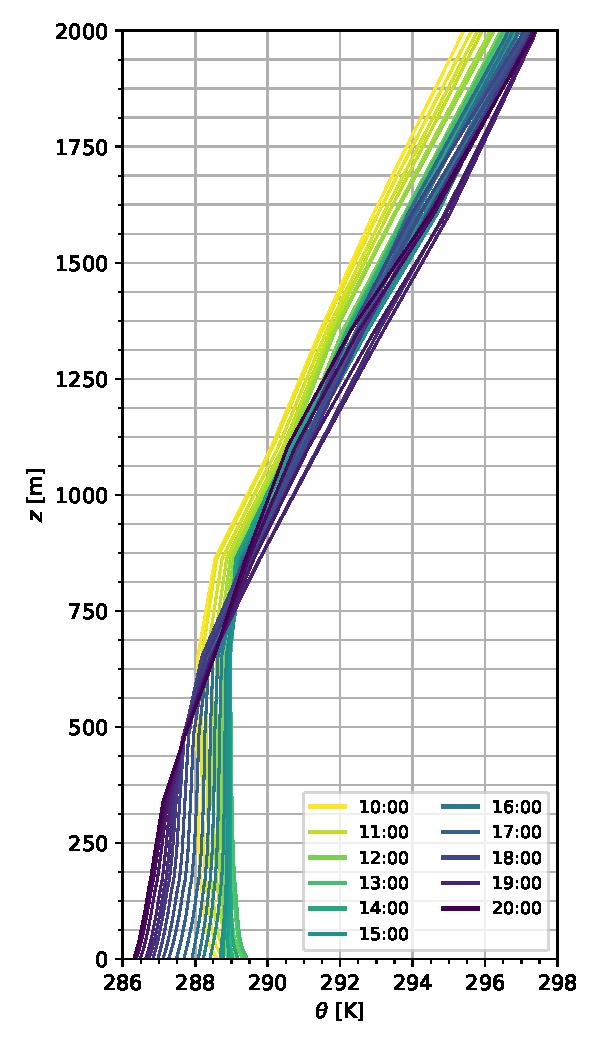
\includegraphics[width=0.86\linewidth,trim={0cm 5mm 0cm 0mm},clip]{Imagenes/06/hov/pbl}%
	\end{minipage}%
	\begin{minipage}{0.5\linewidth}
		\centering
		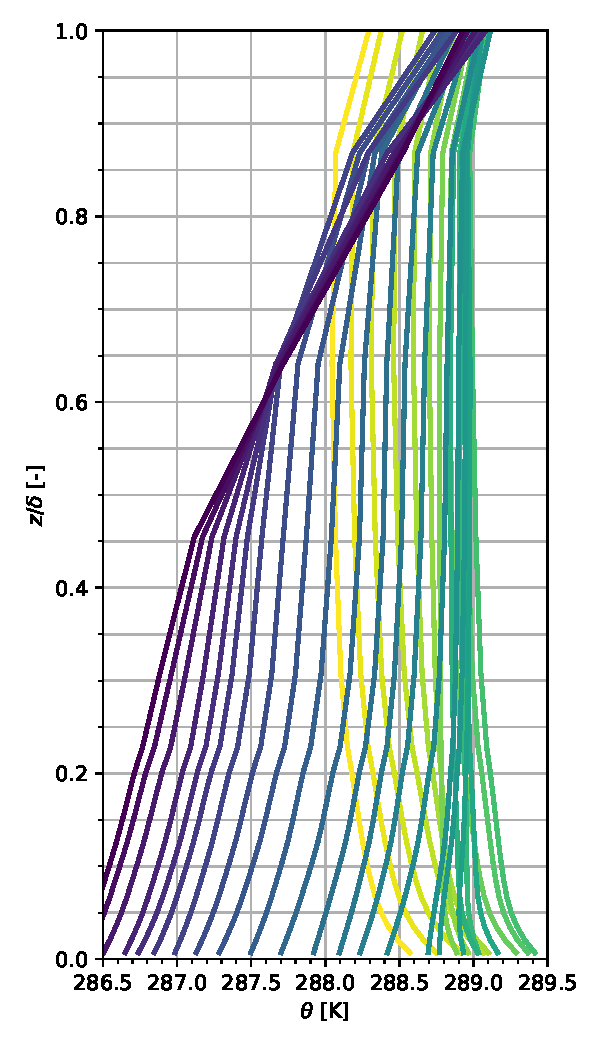
\includegraphics[width=0.86\linewidth,trim={0cm 5mm 0cm 0cm},clip]{Imagenes/06/hov/temp_profile}%
	\end{minipage}%
	
	\caption{Ciclo diurno-nocturno del perfil de temperatura potencial en el mástil meteorológico. (a) Resultados cada 20 minutos del perfil de $\theta_v$. (b) Corresponde al detalle del perfil dentro de la capa límite atmosférica ($\delta \approx 750$ [m]).}
	\label{fig:06_hov_pbl}
\end{figure}

\begin{figure}[H]
	\centering
	\begin{minipage}{0.5\linewidth}
		\center\hspace{0.3cm}(a)
	\end{minipage}%
	\begin{minipage}{0.5\linewidth}
		\center\hspace{0.3cm}(b)
	\end{minipage}%
	
	\includegraphics[width=0.5\linewidth,page=55,trim={2.5cm 6.2cm 1cm 4.5cm},clip]{Imagenes/06/hov/eta1_u}%
	\includegraphics[width=0.5\linewidth,page=55,trim={2.5cm 6.2cm 1cm 4.5cm},clip]{Imagenes/06/hov/eta1_v}%
	
	\center{\hspace{0.3cm}(c)}
	
	\includegraphics[width=0.5\linewidth,page=55,trim={2.5cm 6.2cm 1cm 4.5cm},clip]{Imagenes/06/hov/eta1_vv}%
	\caption{(a) Componente $u$ de la velocidad en el primer nivel de la coordenada vertical ($z_1=5.25$ [m]) para las 15:00. (b) Idéntico al anterior pero para la componente $v$. (c) Magnitud del campo de velocidad.}
	\label{fig:06_hov_eta1}
\end{figure}

\begin{figure}[H]
	\centering
	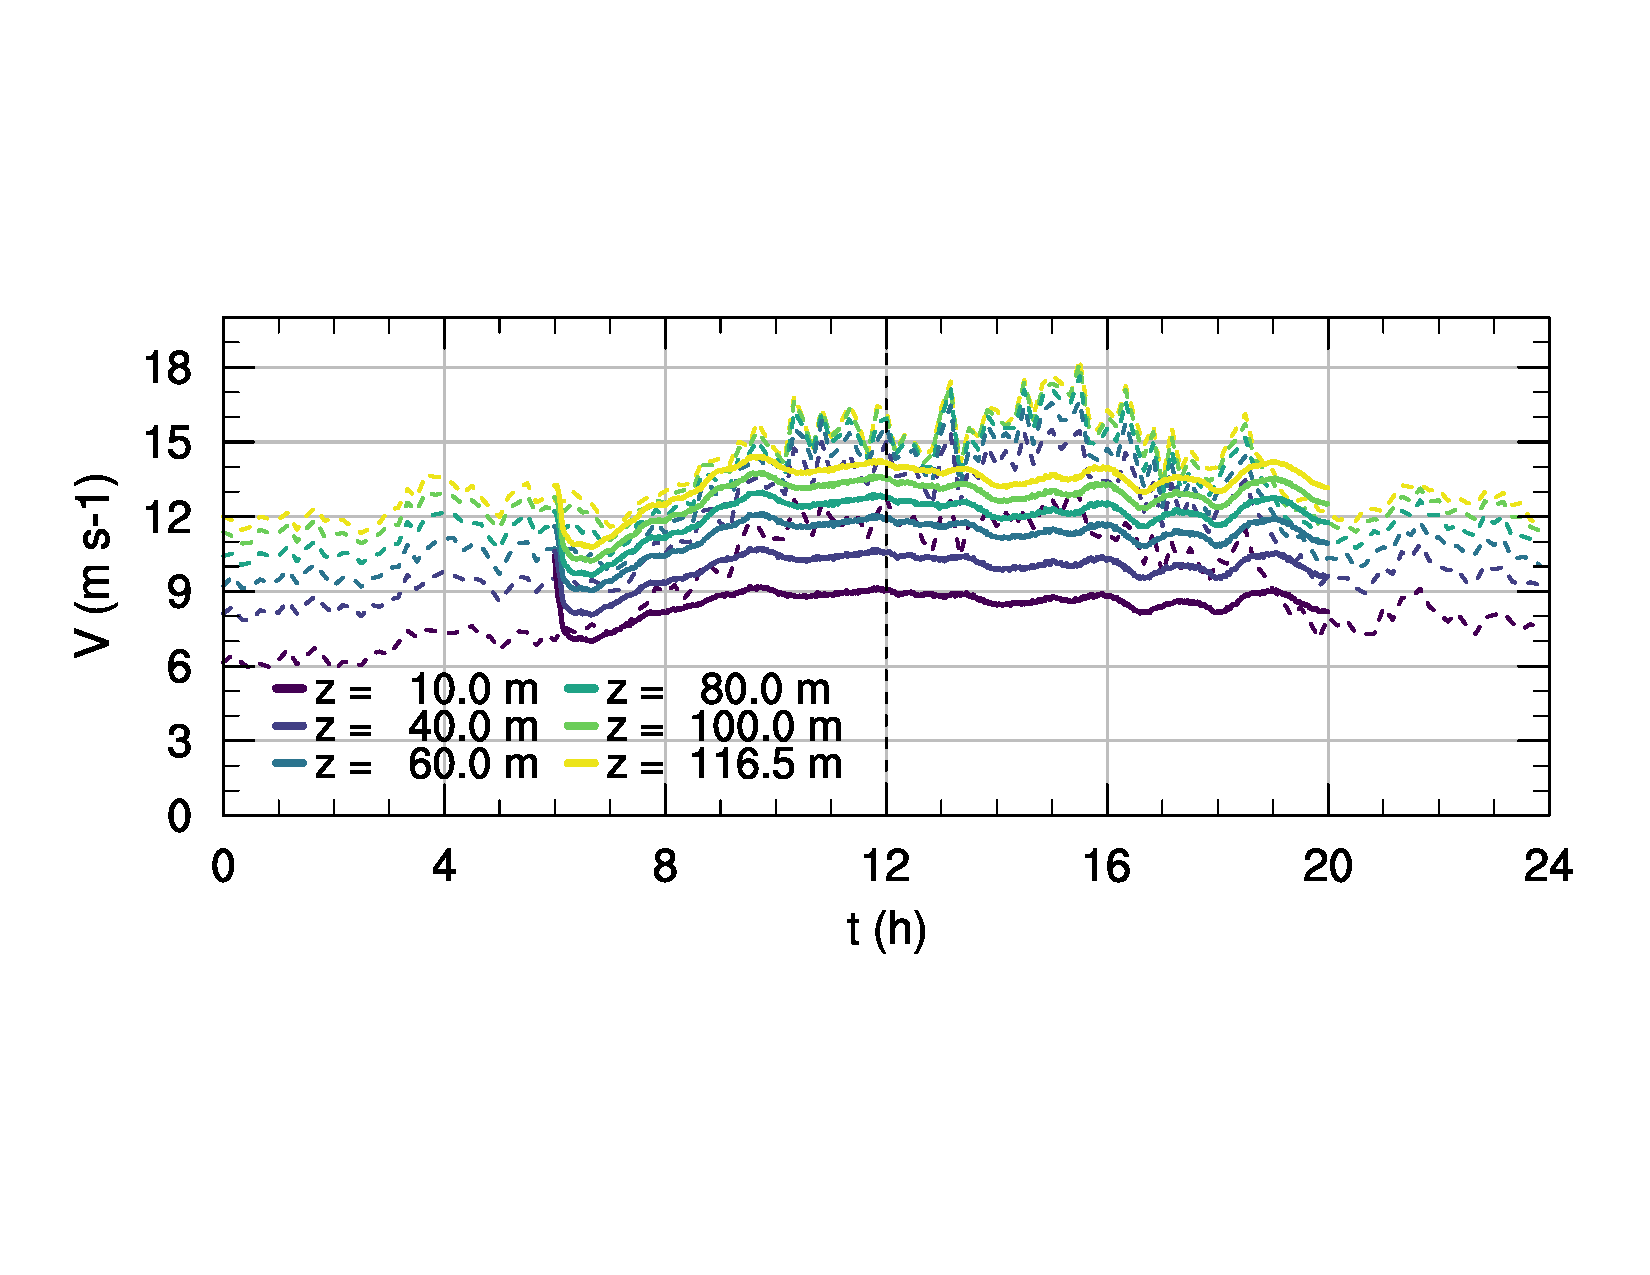
\includegraphics[width=1\linewidth,trim={9mm 63mm 10mm 55mm},clip]{Imagenes/06/hov/ts_v}%
	
	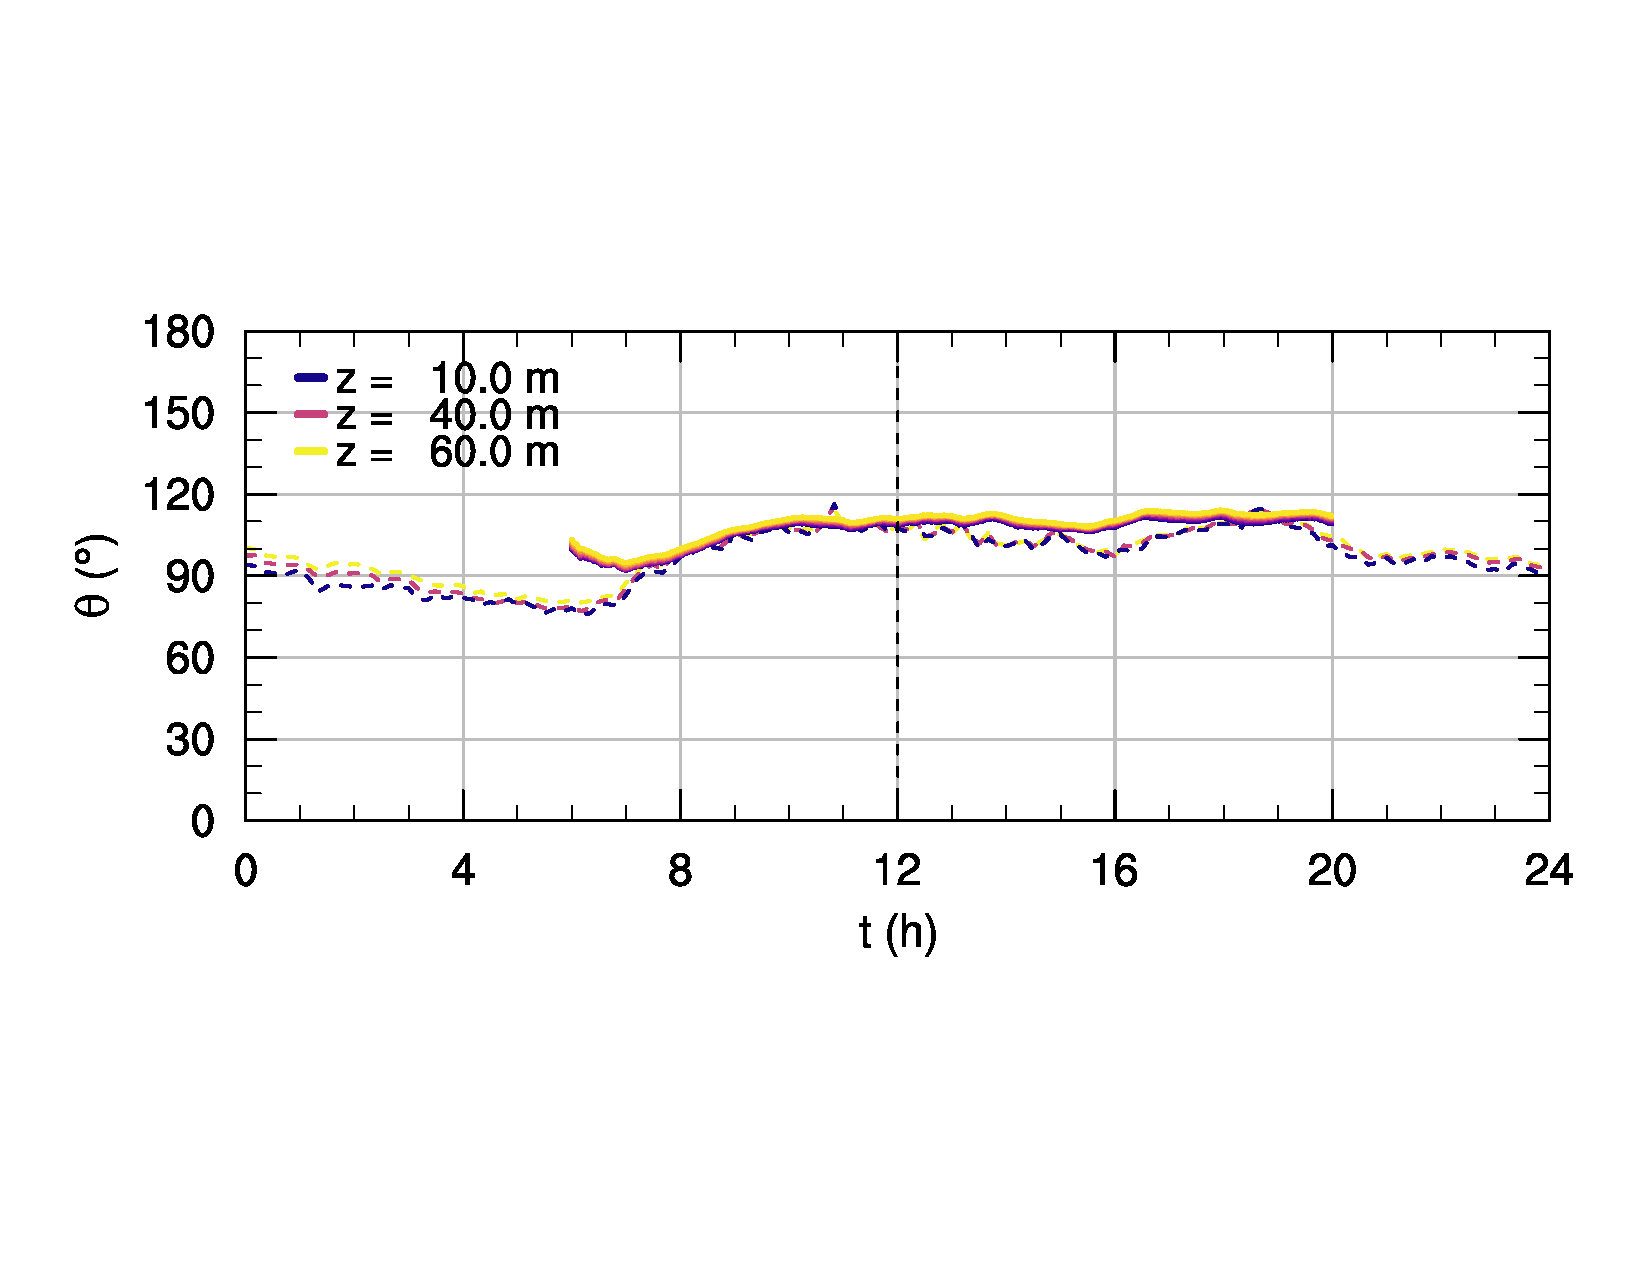
\includegraphics[width=1\linewidth,trim={12mm 55mm 10mm 55mm},clip]{Imagenes/06/hov/ts_o}%
	\caption{Serie de tiempo para la rapidez instantánea del viento $V$ y su dirección en la ubicación del mástil meteorológico. La línea continua corresponde a lo datos simulados interpolados a las alturas de medición (solo para $V$) y la línea punteada a los datos medidos en el mástil.}
	\label{fig:06_hov_ts}
\end{figure}



\begin{figure}[H]
	\begin{minipage}{0.33\linewidth}
		\centering \hspace{1cm}(a)
	\end{minipage}%
	\begin{minipage}{0.33\linewidth}
		\centering \hspace{0.8cm}(b)
	\end{minipage}%
	\begin{minipage}{0.33\linewidth}
		\centering \hspace{0.5cm}(c)
	\end{minipage}%
	\vspace{-4mm}
	\begin{center}
		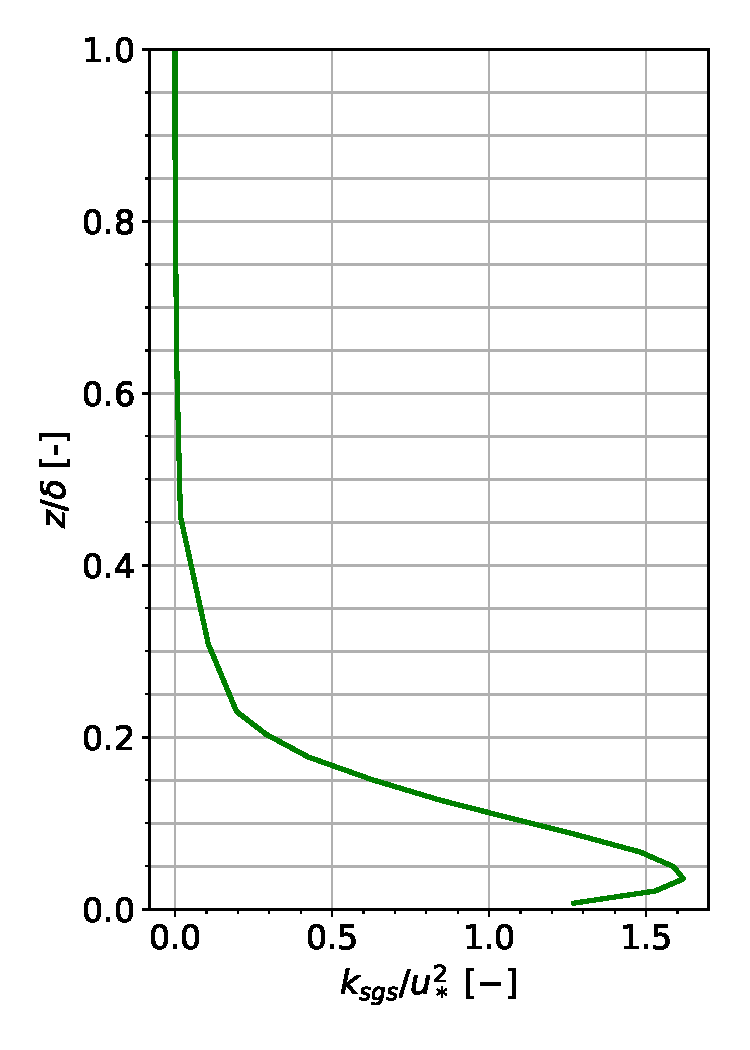
\includegraphics[height=0.5\linewidth,page=1,trim={6mm 5mm 3mm 0mm},clip]{Imagenes/06/hov/mean_data}%
		\includegraphics[height=0.5\linewidth,page=2,trim={12mm 5mm 3mm 0mm},clip]{Imagenes/06/hov/mean_data}%
		\includegraphics[height=0.5\linewidth,page=3,trim={12mm 5mm 3mm 0mm},clip]{Imagenes/06/hov/mean_data}%
	\end{center}
	\caption{Variables adimensionalizadas ($u_* = 0.552$ [m/s]) de segundo orden para el caso de Høvsøre promediados entre las 12:00 y las 15:00 (atmósfera neutra, terreno plano homogéneo). (a) Energía cinética turbulenta de submalla, (b) Gradiente de velocidad, (c) Esfuerzo turbulento. }
	\label{fig:06_hov_mean_secondorder}
\end{figure}

\begin{figure}[H]
	\centering
	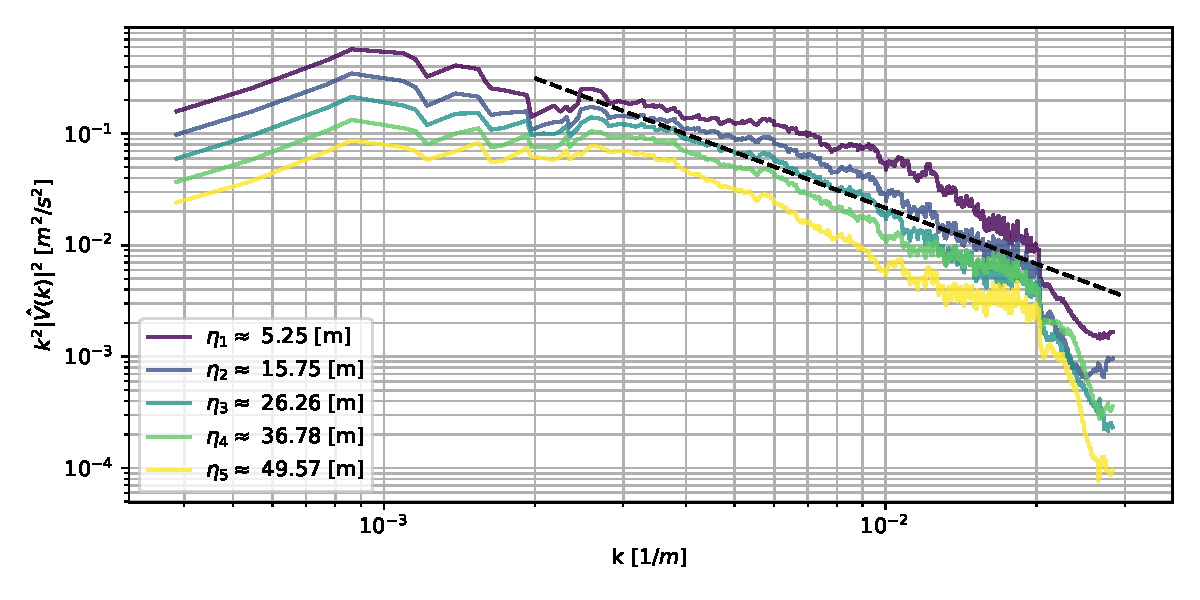
\includegraphics[width=1.0\linewidth,page=1,trim={3mm 5mm 3mm 3mm},clip]{Imagenes/06/hov/spectra}%
	\caption{Espectros de energía para la componente horizontal del viento a distintos niveles verticales en el dominio d07 caso Høvsøre.}
	\label{fig:06_hov_spectrum}
\end{figure}

\begin{figure}[H]
	\centering
	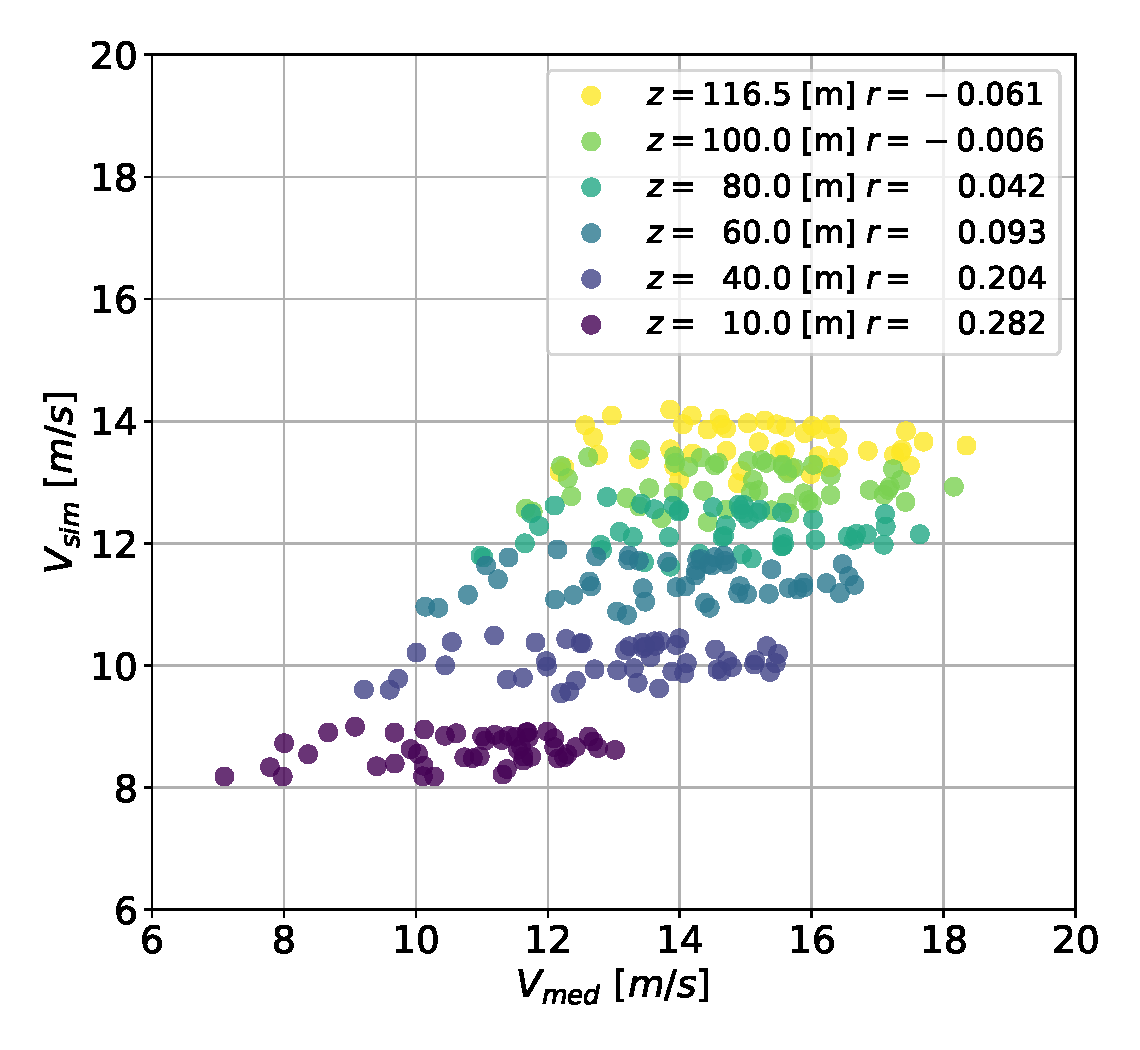
\includegraphics[width=0.55\linewidth,page=1,trim={0cm 0cm 0cm 0cm},clip]{Imagenes/06/hov/corr}%
	\caption{Gráfico de dispersión para las velocidades a distintas alturas en el mástil meteorológico de Høvsøre.}
	\label{fig:06_corr_hov}
\end{figure}

\begin{figure}[H]
	\centering
	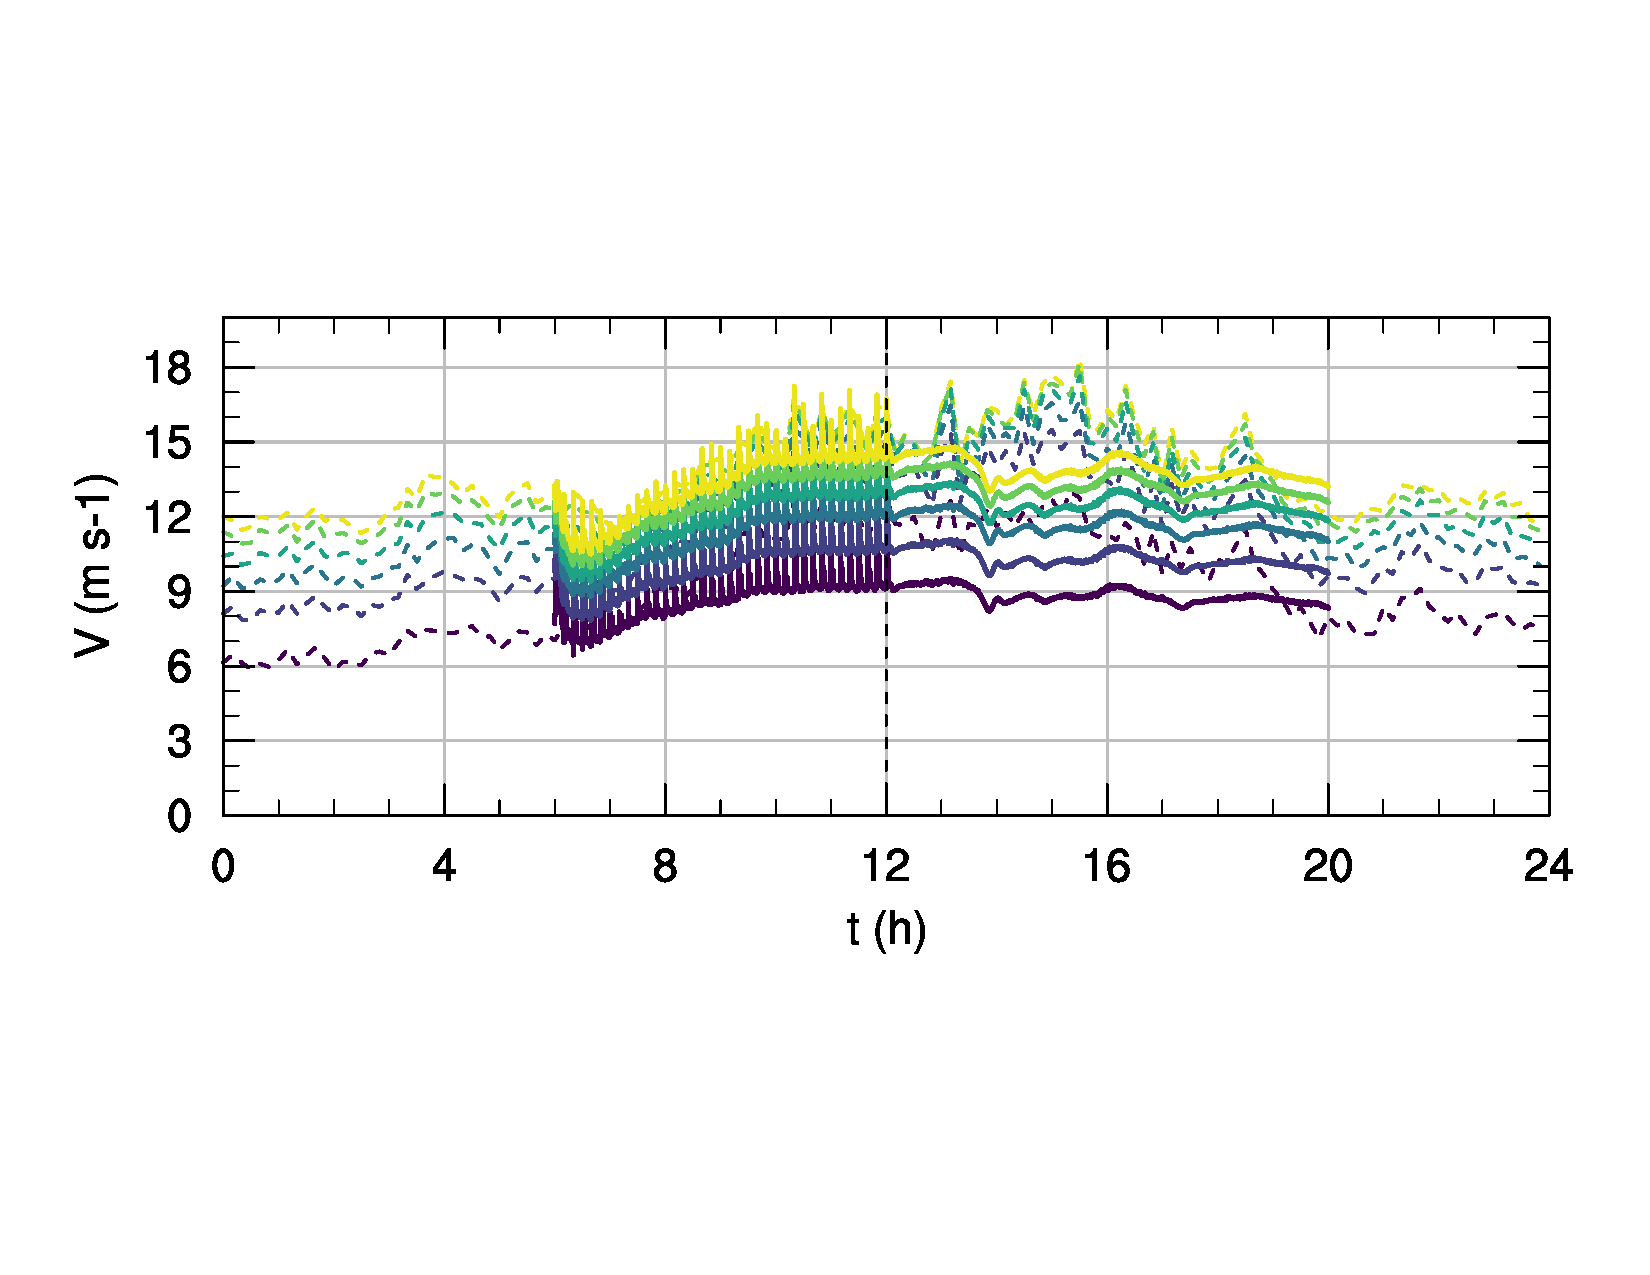
\includegraphics[width=1\linewidth,trim={9mm 63mm 10mm 55mm},clip]{Imagenes/06/hov_da/ts_v}%
	
	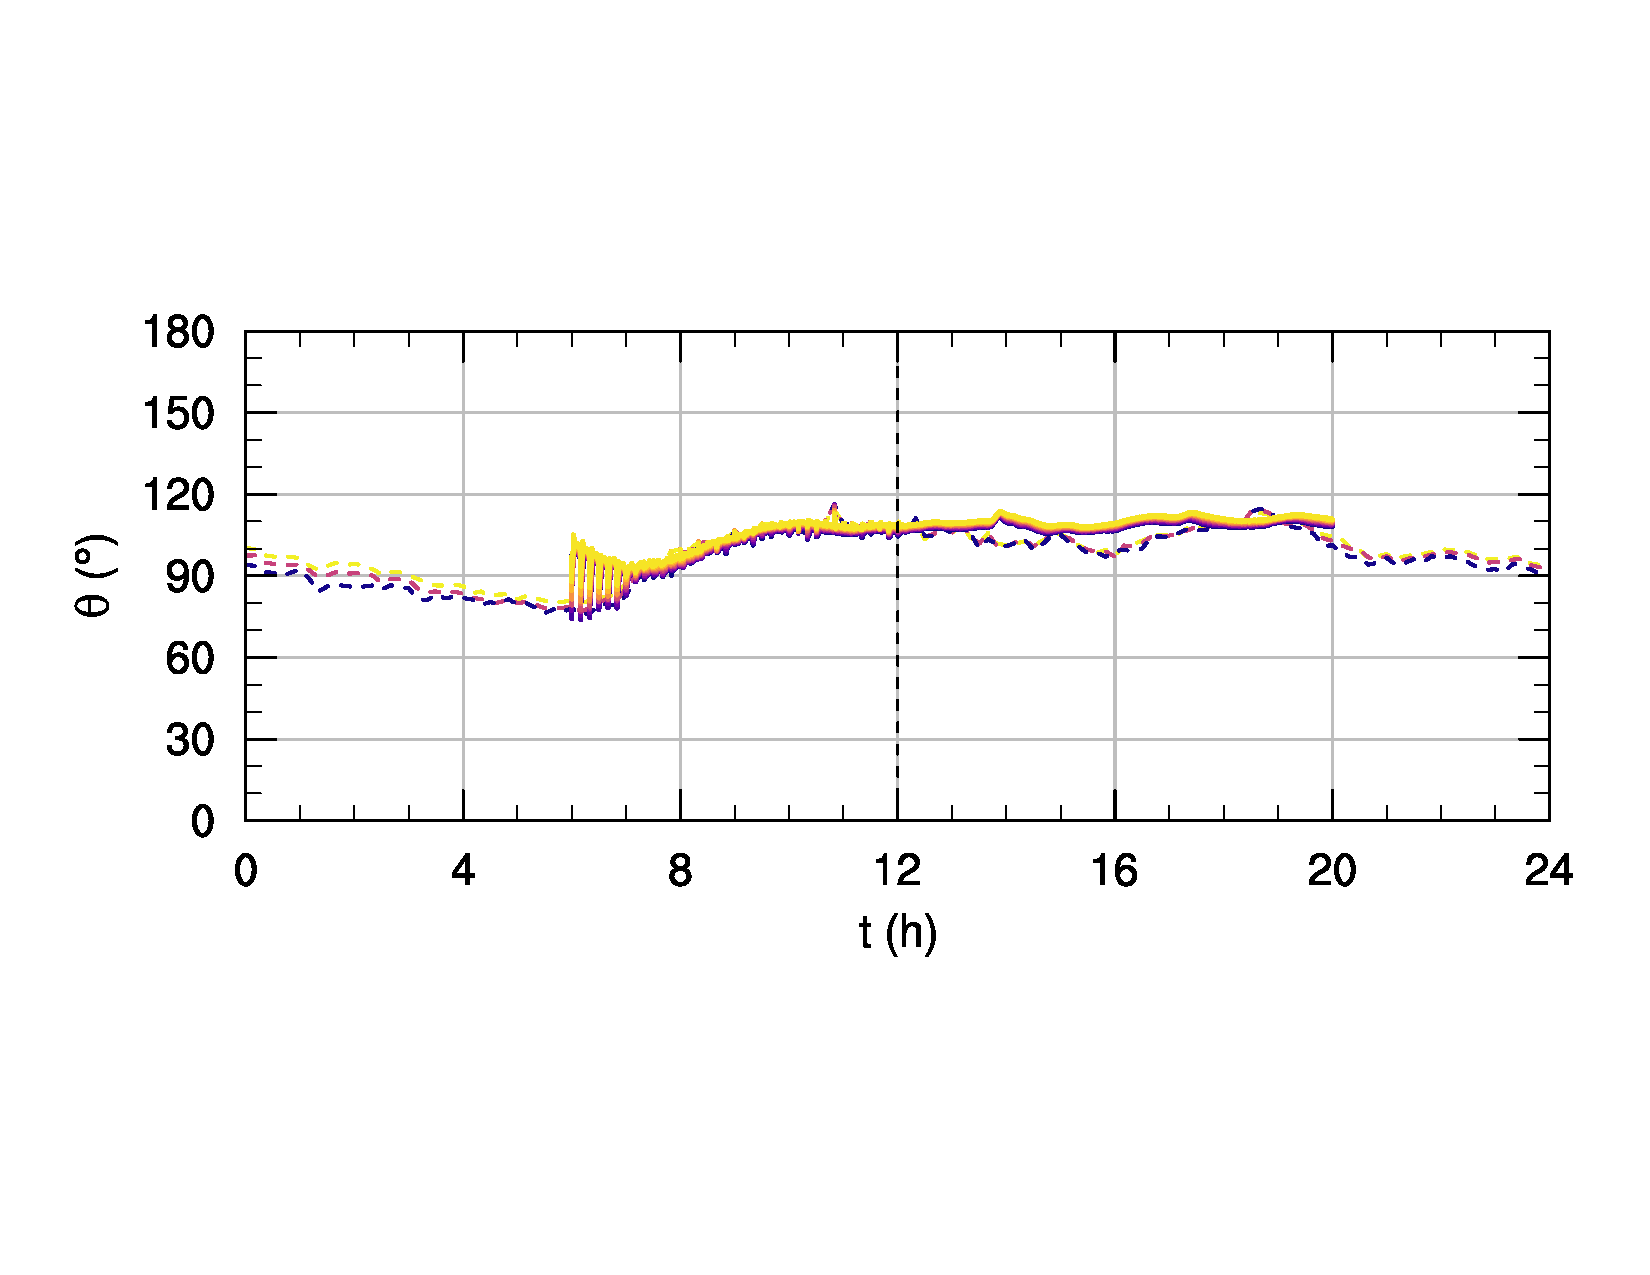
\includegraphics[width=1\linewidth,trim={12mm 55mm 10mm 55mm},clip]{Imagenes/06/hov_da/ts_o}%
	\caption{Serie de tiempo para la rapidez instantánea del viento $V$ y su dirección en la ubicación del mástil meteorológico para el caso con asimilación de datos. La línea continua corresponde a lo datos simulados interpolados a las alturas de medición (solo para $V$) y la línea punteada a los datos medidos en el mástil.}
	\label{fig:06_hov_da_ts}
\end{figure}

\begin{figure}[H]
	\begin{minipage}{0.33\linewidth}
		\centering \hspace{1cm}(a)
	\end{minipage}%
	\begin{minipage}{0.33\linewidth}
		\centering \hspace{0.8cm}(b)
	\end{minipage}%
	\begin{minipage}{0.33\linewidth}
		\centering \hspace{0.5cm}(c)
	\end{minipage}%
	\vspace{-4mm}
	\begin{center}
		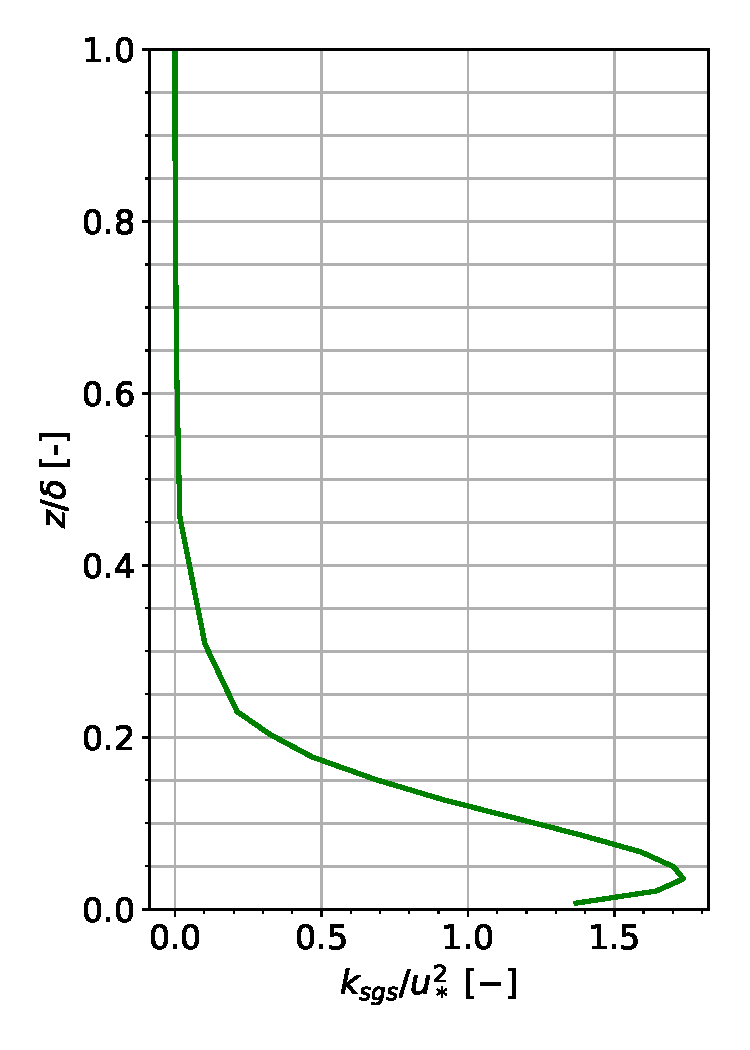
\includegraphics[height=0.5\linewidth,page=1,trim={6mm 5mm 3mm 0mm},clip]{Imagenes/06/hov_da/mean_data}%
		\includegraphics[height=0.5\linewidth,page=2,trim={12mm 5mm 3mm 0mm},clip]{Imagenes/06/hov_da/mean_data}%
		\includegraphics[height=0.5\linewidth,page=3,trim={12mm 5mm 3mm 0mm},clip]{Imagenes/06/hov_da/mean_data}%
	\end{center}
	\caption{Variables adimensionalizadas ($u_* = 0.527$ [m/s]) de segundo orden para el caso de Høvsøre con DA promediados entre las 12:00 y las 15:00 (atmósfera neutra, terreno plano homogéneo). (a) Energía cinética turbulenta de submalla, (b) Gradiente de velocidad, (c) Esfuerzo turbulento. }
	\label{fig:06_hov_da_mean_secondorder}
\end{figure}

\begin{figure}[H]
	\centering
	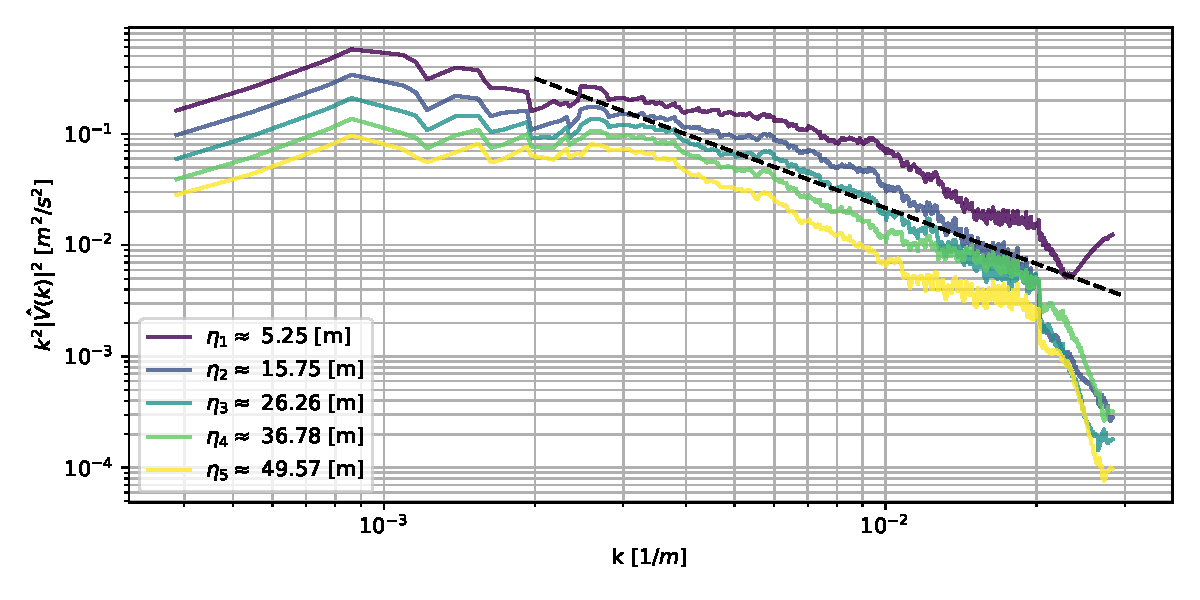
\includegraphics[width=1.0\linewidth,page=1,trim={3mm 5mm 3mm 3mm},clip]{Imagenes/06/hov_da/spectra}%
	\caption{Espectros de energía para la componente horizontal del viento a distintos niveles verticales en el dominio d07 caso Høvsøre con DA.}
	\label{fig:06_hov_da_spectrum}
\end{figure}

\begin{figure}[H]
	\centering
	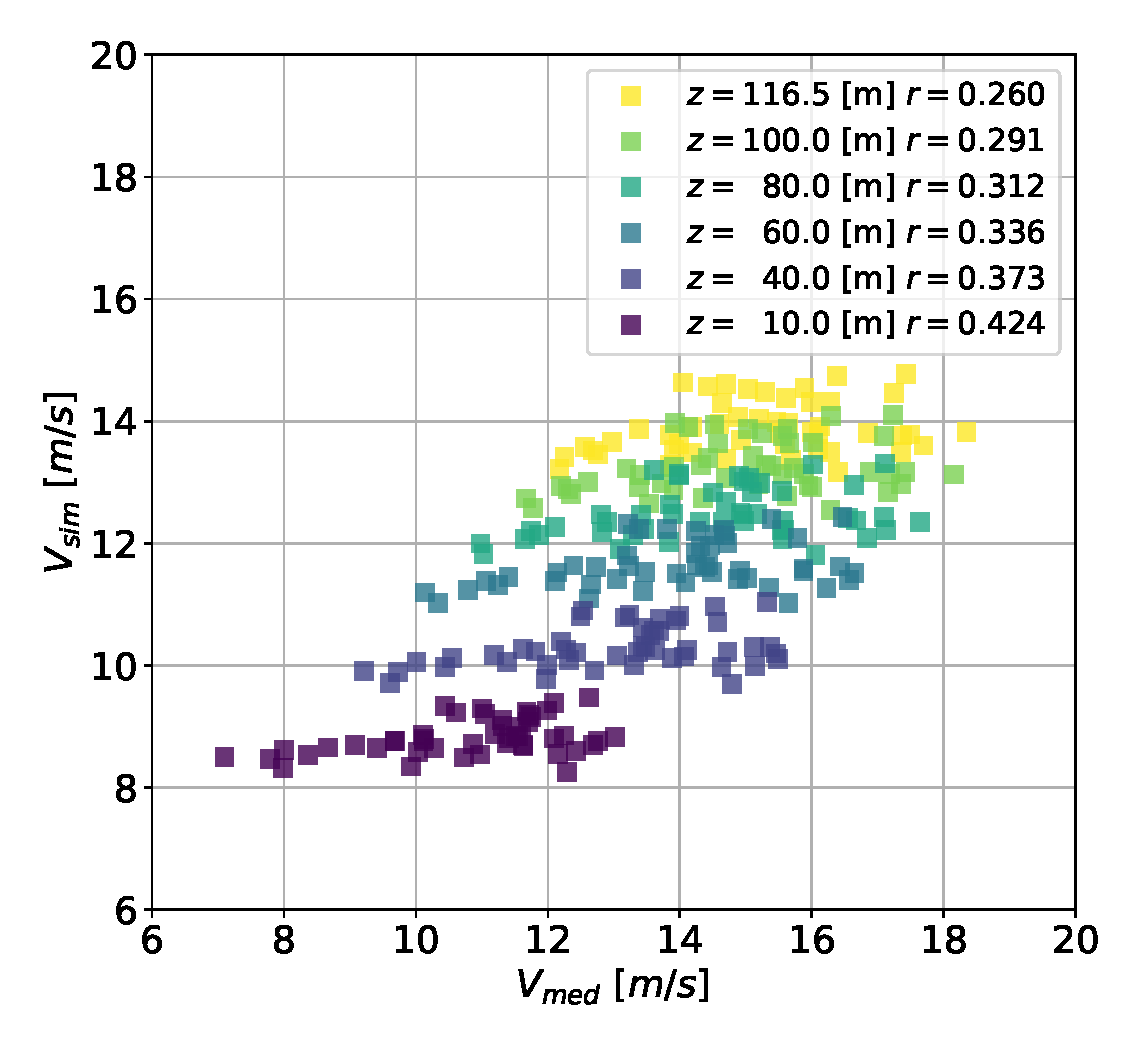
\includegraphics[width=0.55\linewidth,page=1,trim={0cm 0cm 0cm 0cm},clip]{Imagenes/06/hov_da/corr}%
	\caption{Gráfico de dispersión para las velocidades a distintas alturas en el mástil meteorológico de Høvsøre (con DA).}
	\label{fig:06_corr_hov_da}
\end{figure}

\begin{table}[H]
	\caption{Comparación de métricas para el caso I Høvsøre.}
	\label{tab:06_hov_mae_rmse}
	\centering%\footnotesize
	\begin{tabular}{lcc}
		\toprule
		& Sin DA & Con DA \\
		\midrule
		MAE & 2.41091 m/s & 2.16742 m/s \\
		RMSE & 2.80142 m/s& 2.55778 m/s\\
		$\Delta{RMSE}$& --  & $8.70\%$  \\
		$\Delta{MAE}$ & -- & $10.47\%$  \\
		\bottomrule
	\end{tabular}
\end{table}